\chapter{Stochastic Tractography}
\begin{figure} \label{fig:stflow}
  \center 
	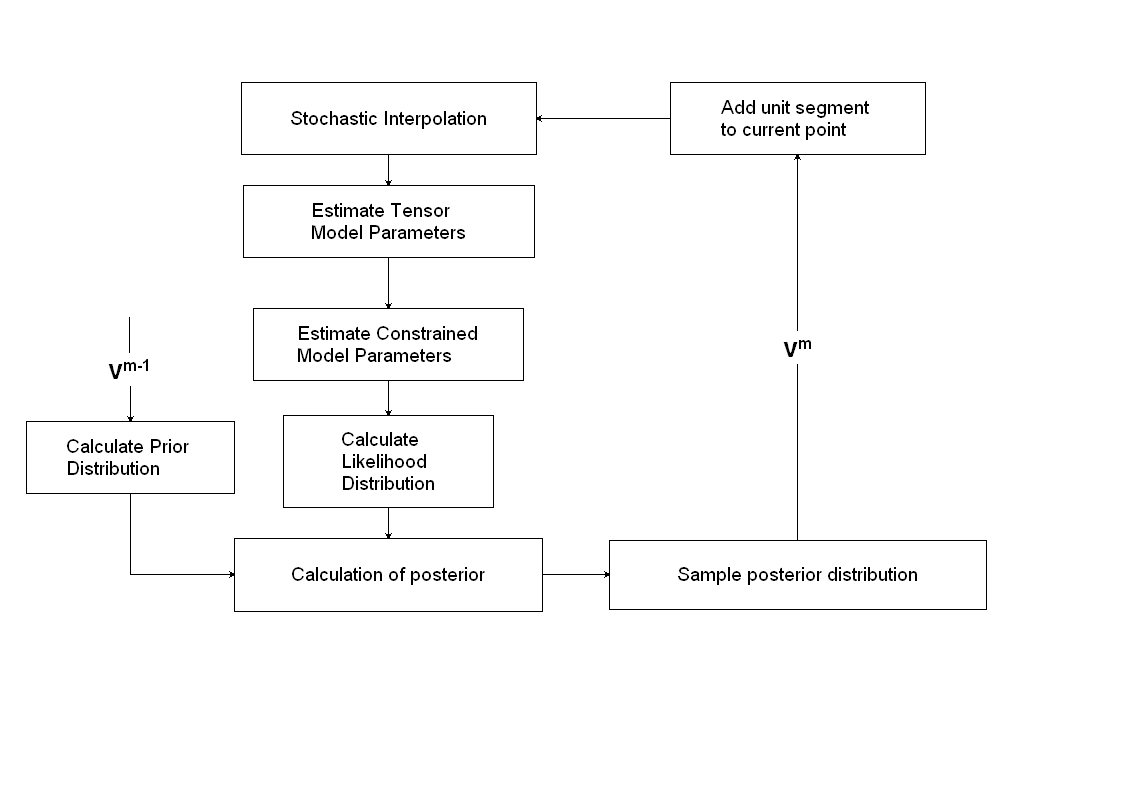
\includegraphics[trim = 10mm 50mm 20mm 30mm, clip, width=\linewidth]{stflow}
	\caption{A flow chart demonstrating key steps in the stochastic tractography algorithm}
\end{figure}
The Stochastic Tractography System implemented in this research implements Friman's \cite{frimanTMI06} approach to Stochastic Tractography with some modifications to the stopping criteria.  Figure \ref{fig:stflow} provides a flow chart demonstrating key steps in the algorithm.  A brief explanation of the algorithm is given in this section with a detailed derivation given in appendix A.

A fiber tract is modeled as a train of unit vectors.  The orientation of these unit vectors are determined by sampling a posterior fiber orientation distribution which is dependent on the local diffusion data as well as the orientation of the unit vector in the previous step.  The posterior distribution is a normalized product of the prior likelihood of the fiber orientation and the likelihood of that fiber orientation given the local diffusion data.

Friman uses a subset of the tensor model which is called a constrained diffusion model.  In this model, the two smallest eigenvectors of diffusion tensor are equal, constraining the shape of the diffusion tensor to be linearly anisotroopic.  The constrained model rules out the possibility of nonlinear, or non-cylindrical anisotropic diffusion distributions.  Deviations from linearly anisotropic diffusion distributions are captured as uncertainty in the fiber orientation.  The constrained model is combined with a Gaussian DWI noise model to obtain a fiber orientation likelihood function.  The parameters for the constrained model are derived from a WLS estimation of the parameters for the tensor model.

The orientation of each vector depends only on the previous vector.  This dependency is formulated in the prior on the fiber orientation.  Prior knowledge about the regularity of the fiber tract can encoded in this prior probability.  The prior also serves to prevent the fiber from backtracking, since the likelihood distribution alone is axially symmetric.

Friman's approach is a Bayesian based inference algorithm similar to Behren's but with some optimizations to Behren's approach \cite{frimanTMI06}.  In contrast with Behren's two-compartment observation model, the constrained model used by Friman is derived from the thoroughly studied tensor model of diffusion.  The advantage of using the constrained model is that it is relatively easy to estimate the parameters for the model.  The parameters for the constrained model are obtained easily after the tensor model has been fit to the diffusion data.  Since the parameters for the tensor model are easily obtained through many computationally efficient ways, the constrained model's parameters are likewise easy to obtain.  The constrained model is able can be fit to every voxel within a matter of seconds whereas Behren model takes a couple of hours \cite{frimanTMI06}.  Additionally Friman avoids using MCMC techniques by assuming that parameters other than the principle diffusion direction take on their ML estimates with certainty within each voxel.  Friman demonstrates that eliminating this source of uncertainty has little effect on the resulting posterior fiber orientation distribution.

In Friman's paper on stochastic tractography, the tracking was terminated when an encountered voxel was too isotropic.  However, since the stochastic tractography algorithm takes into account this uncertainty with an increase in the spatial variance of sampled fibers, this termination criteria seems arbitrary and contradictory with the goals of stochastic tractography, which is to enable sampling of tracts in regions of uncertainty.  Thus this termination criteria has been replaced with a criteria which terminates tractography based on posterior probability that a fiber tract exists within the current voxel.  The posterior probability that a fiber tract exists in a given voxel can be obtained by performing a soft segmentation of white matter on an anatomical image co-registered with the DWI data.  Alternatively, the soft segmentation can also be performed on the B0 image of the DWI data set, thus eliminating the need for additional data.  Although this may seem equivalent to using fractional anisotropy since white matter generally has higher anisotropy than gray matter, it does not exclude isotropic regions of white matter which have crossing fibers.  Theoretically, this criteria should enable the algorithm to detect more tracts than under the anisotropy termination criteria.
%talk through key portions of the math
%present a block diagram of the algorithm




%need to add in a bit about how they are different in the way they sample the PDF

%talk about how it differs from other algorithms
%talk about using incorporating the posterior probability of white matter
%talk about why we choose to segment the gray/white matter using b0 image instead of using diffusion information
